%
% teil3.tex -- Beispiel-File für Teil 3
%
% (c) 2020 Prof Dr Andreas Müller, Hochschule Rapperswil
%
% !TEX root = ../../buch.tex
% !TEX encoding = UTF-8
%
\subsection{Kreuzung 
\label{genetic_algorithm:crossover}}
In diesem Teil des Algorithmus werden die gewählten Elternpaare 
neu kombiniert, um Nachkommen zu erzeugen. Bei der Kreuzung 
werden Teile des genetischen String ausgetauscht.

\begin{figure} [h]
	\centering
	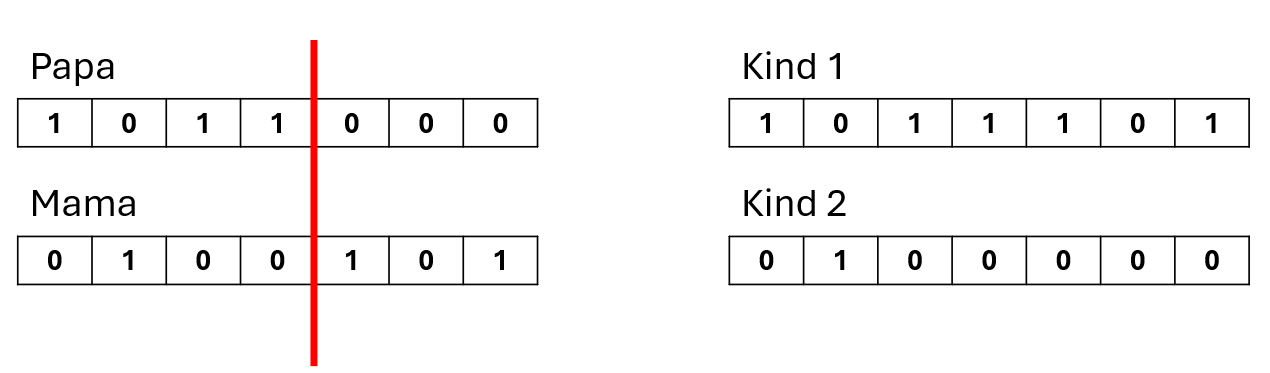
\includegraphics[width=0.8\textwidth]{
        papers/variationsprinzip_algorithmen/images/teil3/05_genetic_string_cross.png
        }
	\caption{Ein einfaches Beispiel für eine Einpunkt-Kreuzung}
	\label{fig:one_point_crossover}
\end{figure}

Für die Kreuzung gibt es unterschiedliche Taktiken:

- **Einpunkt-Kreuzung:** Ein zufälliger Punkt wird auf den 
Elternchromosomen ausgewählt. Die Gene vor diesem Punkt 
stammen vom ersten Elternteil, die Gene nach diesem Punkt 
vom zweiten Elternteil. Mathematische:\\
Wähle einen zufälligen Punkt \( k \) (1 ≤ k < n).\\
Erzeuge die Nachkommen durch:
\[ O_1 = (P_1[1], P_1[2], \ldots, P_1[k], P_2[k+1], \ldots, P_2[n]) \]
\[ O_2 = (P_2[1], P_2[2], \ldots, P_2[k], P_1[k+1], \ldots, P_1[n]) \]
\\
- **Zweipunkt-Kreuzung:** Zwei Punkte werden ausgewählt und 
der Genabschnitt zwischen diesen Punkten wird zwischen 
den Eltern getauscht.\\
Wähle zwei zufällige Punkte \( k_1 \) und \( k_2 \) (1 ≤ k_1 < k_2 < n).\\
Erzeuge die Nachkommen durch:
\[ O_1 = (P_1[1], \ldots, P_1[k_1], P_2[k_1+1], \ldots, P_2[k_2], P_1[k_2+1], \ldots, P_1[n]) \]
\[ O_2 = (P_2[1], \ldots, P_2[k_1], P_1[k_1+1], \ldots, P_1[k_2], P_2[k_2+1], \ldots, P_2[n]) \]
\\
- Uniforme Kreuzung: Jedes Gen wird mit einer bestimmten 
Wahrscheinlichkeit vom ersten oder zweiten Elternteil 
übernommen, was zu einer zufälligeren Kombination führt.
Mathematische Formel:\\
Für jedes Gen \( i \) (1 ≤ i ≤ n):\\
Wähle eine zufällige Zahl \( r_i \) im Intervall [0, 1].\\
Wenn \( r_i \) kleiner als die vordefinierte Wahrscheinlichkeit 
\( p \) ist, dann wird das Gen von \( P_1 \) übernommen, 
ansonsten von \( P_2 \).

\[ O_1[i] = 
\begin{cases} 
P_1[i] & \text{wenn } r_i < p \\
P_2[i] & \text{wenn } r_i \geq p 
\end{cases} \]

\[ O_2[i] = 
\begin{cases} 
P_2[i] & \text{wenn } r_i < p \\
P_1[i] & \text{wenn } r_i \geq p 
\end{cases} \]

Hier wird die Variation aufrechterhalten (Grösse der Population
bleibt gleich gross) und gleichzeitig wird aus den besten Genen 
neue erstellt, mit dem Versuch noch besseres Resultat zu bekommen.

Wie schon in der Initialisierung erwähnt, kann nicht ein normaler 
genetischer String \ref{fig:one_point_crossover} mit An und 
Aus verwendet werden. Dies würde zu einem Resultat wie in der Abbildung 
\ref{fig:one_point_crossover_cities} führen.

\begin{figure} [h]
	\centering
	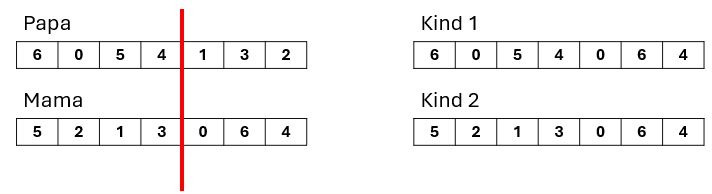
\includegraphics[width=0.8\textwidth]{
        papers/variationsprinzip_algorithmen/images/teil3/07_genetic_string_cities_crossover_standard.png
        }
	\caption{Beispiel einer Einpunkt-Kreuzung mit Städten}
	\label{fig:one_point_crossover_cities}
\end{figure}

Für das Travelings Salesman Problem wird die Kreuzung mit andern Systemen 
angepasst, damit es keine Doppelten gibt.

Für den Script wurden die Logik angepasst. Die Algorithmen entfernen einen 
Teil des Strings, wie bei in den vorherigen Kreuzungen, aber es fügt nach 
der Reihenfolge des zweiten Elternteils alle nicht vorhandenen 
Städte hinzu, bis der herausgeschnittene String wieder vollständig ist.

\begin{figure} [h]

\begin{figure} [h]
	\centering
	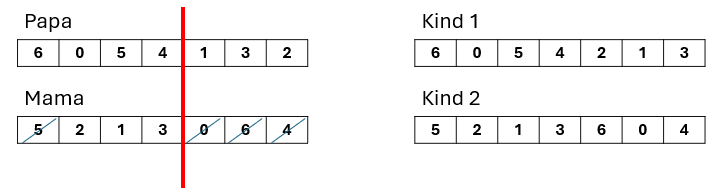
\includegraphics[width=0.8\textwidth]{
        papers/variationsprinzip_algorithmen/images/teil3/08_genetic_string_cities_crossover_simple.png
        }
	\caption{Beispiel einer Einpunkt-Kreuzung mit Städten}
	\label{fig:crossover_order_cities}
\end{figure}

